\documentclass{standalone}

\usepackage[euler-digits]{eulervm}

\usepackage{tikz}
\tikzset{every node/.style={shape=circle,draw=none,fill=blue,minimum size=1.5mm,inner sep=0pt}}

\begin{document}
\begin{tabular}{c|c|c}
  $T$ & $\#\mathrm{Aut}(T)$ & $\#S(T)$ \\ \hline
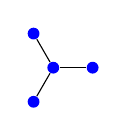
\begin{tikzpicture}[scale=0.5,baseline=-1mm]
      \node (0) at (0,0) {};
      \node (1) at (0:1) {};
      \node (2) at (120:1) {};
      \node (3) at (240:1) {};
\foreach \y in {1,2,3}
  \draw (0) -- (\y);
\end{tikzpicture} & $6$ & $4$ \\
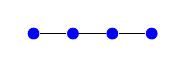
\begin{tikzpicture}[scale=0.5,baseline=4mm]
      \node (0) at (0,1) {};
      \node (1) at (1,1) {};
      \node (2) at (2,1) {};
      \node (3) at (3,1) {};
\foreach \x/\y in {0/1,1/2,2/3}
  \draw (\x) -- (\y);
\end{tikzpicture} & $2$ & $12$ \\ \hline
\end{tabular}
\end{document}
